%!TEX root = ../../main.tex


\begin{figure}[!htb]
%{\smaller\texthv{\textbf{A. Simulated sample}}}\\
%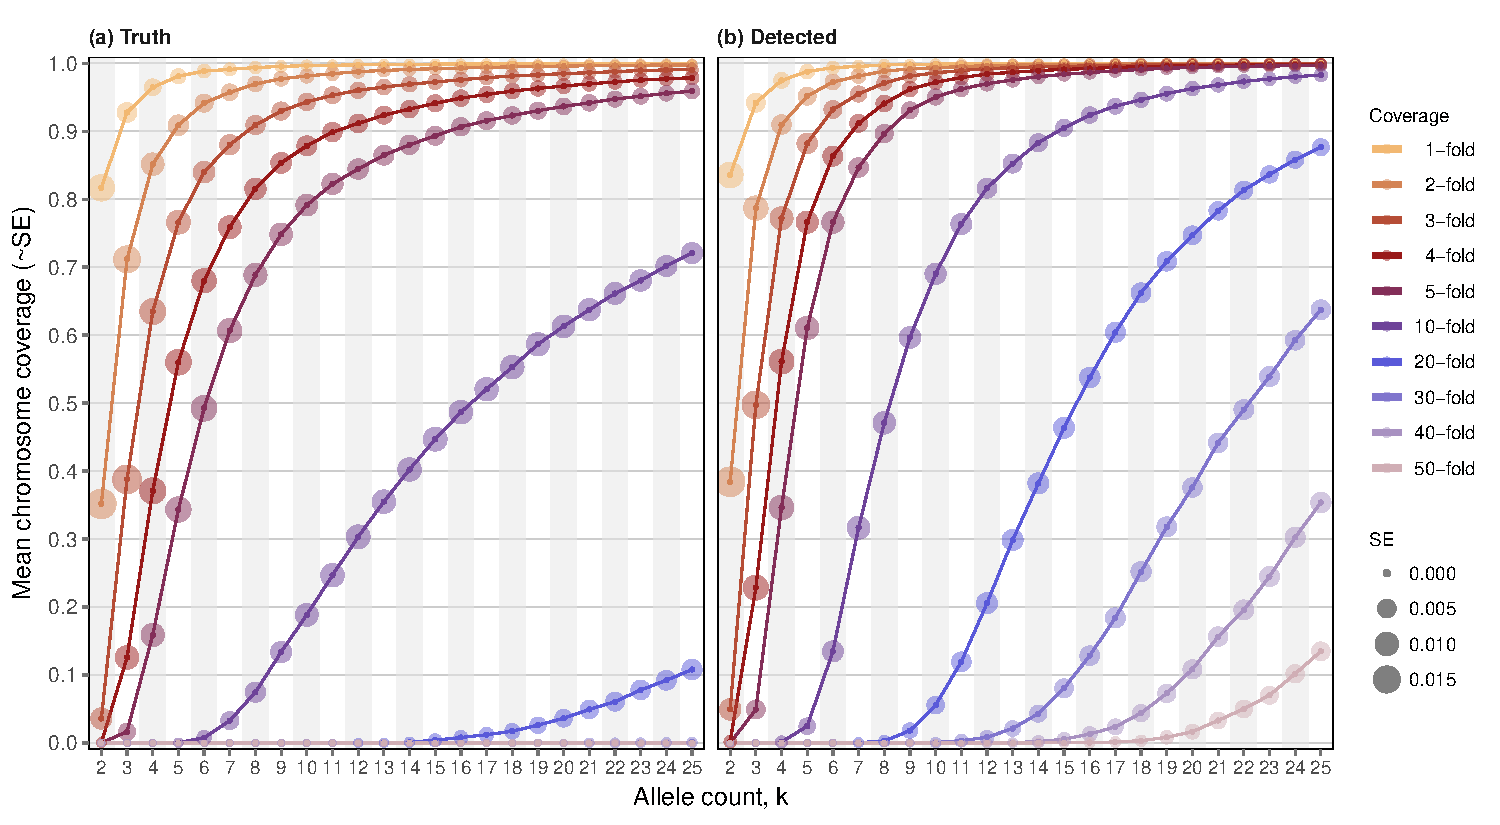
\includegraphics[width=\textwidth]{./img/ch3/phase_fk_coverage}
%{\smaller\texthv{\textbf{B. 1000 Genomes, chromosome 20}}}\\
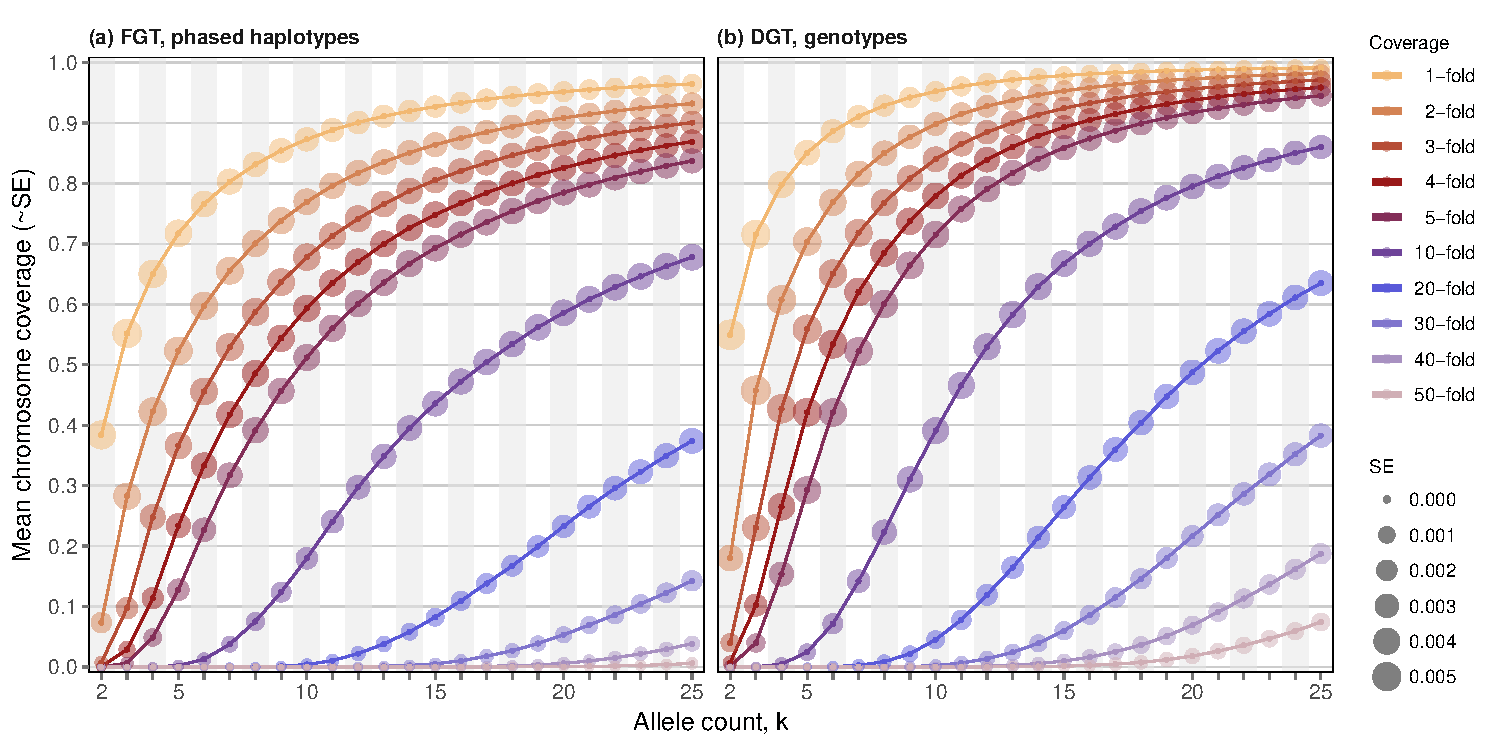
\includegraphics[width=\textwidth]{./img/ch3/phase_coverage_1kg}
\Caption{Cumulative shared haplotype coverage by focal allele count in 1000 Genomes data}
{Results are shown for \n{500} randomly selected individuals, among ${N=\num{2504}}$ in the \gls{1kg} dataset.
% (\textbf{A}), and among the ${N=\num{2504}}$ individuals in 1000 Genomes data, chromosome~20 (\textbf{B}).
Segments detected using the \gls{fgt} (\text{a}, \emph{left}) are compared to the segments detected using the \gls{dgt} (\text{b}, \emph{right}).
%In~B, for comparison, the \gls{fgt} is compared to the \gls{dgt} in the 1000 Genomes dataset.
Coverage was defined as the proportion of chromosome length covered by inferred and aligned shared haplotypes, where $n$-fold indicates that the chromosome was covered $n$-times by all segments up to a given \fk{}~category (hence, cumulative).
\Gls{se} is indicated by the size of dots (see figure legend).}
{fig:phase_fk_coverage}
\end{figure}
